\chapter{MCC - Mission Control Center}\label{MCC - Mission Control Center}

\section{Statusorientierter Ablauf}

Um die Lösung der Aufgabe zu strukturieren, aber auch um die Möglichkeit zu haben, die Mission in Teilaufgaben zu unterteilen, ist der Ablauf grundsätzlich in 5 verschiedene Status unterteilt. Jeder einzelne Status besteht aus einem definierten Ziel und dementsprechend Abbruch-, bzw. Abschlusskriterien. Die Implementierung ist in Form einer ``META-State-Machine'' vorgenommen, die den (inneren) Status der Mission kennt und bei Änderung diesen an die einzelenen Teilsysteme propagiert. Die im folgenden beschriebenen Status geben die konzeptionellen Bedingungen und Aktionen innerhalb dieses Status wieder, es werden jedoch keine konkreten Abläufe, bzw. Implementierungen dieser Aktionen erläutert. Eine genaue Beschreibung der Abläufe wird in späteren Kapiteln nachgeholt. Die einzelnen von der State-Machine verwalteten Status sind:

\begin{enumerate}
\item Initial
Der Initial-Zustand wird automatisch von allen (Teil-)Systemen zu Beginn der Mission eingenommen ohne von der State-Machine propagiert werden zu müssen. Der Initial-Zustand stellt grundsätzliche einige Vorbedingungen sicher, damit die eigentliche Mission gestarted werden kann. Damit die Kalibirerung (s. u.) der NXT's durch den NAO möglichst geringe Fehler produziert, wird zunächst der NAO aufgestellt (falls er nicht bereits steht) und anschließend mit Hilfe von zwei NXT's auf eine Position innerhalb der Karte kalibriert. Anhand dieser Daten werden auch die Positionen der NXT's bestimmt - sollte es noch weitere NXT's geben, werden diese im Abschluss ebenfalls kalibriert. Für den Übergang in den nächsten Status muss der NAO stehen und alle NXT's und der NAO müssen kalibriert sein.

\item Autonomic Exploration
Die Autonomic Exploration ist die erste Phase in der das unbekannte Gebiet erkundet wird. Zur Erkundung verwenden die NXT's verschiedene Explorationsalgorithmen (s. dazu die Kapitel zum NXT) mit dem Ziel, innerhalb einer vorgegebenen Zeit einen möglichst großen Bereich zu erkunden. Die zeit die für diese Phase veranschlagt ist beträgt 5:00 Minuten. Dieser Wert ist allerdings sehr von der gestellten Aufgabe abhängig - je nach Größe des zu erkundenden Gebietes sollte der Wert entsprechend angepasst werden, damit nach Ablauf der Zeit ein adequater Bereich erkundet wurde.

\item Guided Exploration
In dieser Phase wird zielgerichtet versucht, nicht erkundete Gebiete von den NXT's abfahren zu lassen. Da nicht bekannt ist, wie groß das gesamte zu erkundende Gebiet ist oder welche Ausmaße es hat, muss man Areale, die noch abgefahren werden sollen, nach gewissen Kriterien aussuchen (s. hierzu Geführte Erkundung). Die Punkte die dann letztendlich noch abgefahren werden sollen, werden direkt vom MCC an die entsprechenden NXT's geschickt. Maßgeblich für den Übergang in die nächste Phase ist, dass das Ziel gefunden wurde. Mögliche Adaptionen sind bei Kenntnis des Gebietsumfangs die Erkundung bis ein bestimmter Schwellwert an erkundetem Gebiet relativ zum Gesamtgebiet überschritten wird und das Vorhandensein eines ausreichend großen Weges zum Ziel.

\item Path Verification
Nach der zweiten Erkundungsphase wird der vom MCC berechnete Pfad zum Ziel (s. hierzu Pfad zum Ziel) durch einen NXT verifiziert. Es soll dabei sichergestellt werden, dass der berechnete Weg ausreichende Ausmaße hat, um vom NAO abgelaufen zu werden. Sollte der Weg als ungenügend erkannt werden, wird zur vorigen Phase zurück gesprungen. In dieser kann zielgerichtet versucht werden entweder den berechneten Pfad zu ändern, einen Neuen zu finden oder ein größeres Gebiet zu erkunden, um neue Wege zu finden.

\item NAO Walk
In der letzten Phase wird der NAO von einem NXT zum Ziel geführt. Der NXT wird dabei vom NAO als Fixpunkt genutzt und bewältigt die Strecke abschnittsweise (s. hierzu NAOWalk).
\end{enumerate}

\section{Architekturmodell}
Bevor eine grobe Architektur entworfen werden kann, muss man sich klar machen, welche Funktionen das zu implementierende Stück Software leisten soll. Aus der Anforderungserhebung geht hervor, dass eine Karte existieren muss, in die die erhaltenen Erkundungsinformationen des NXT eingetragen werden können und die in vereinfachter Form an die NXT's geschickt werden kann. Zusätzlich ist es hilfreich, wenn auch nicht zwingend gefordert, dass während des Missionsablaufs die aktuelle gesamte Karte visualisiert wird, um den Missionsfortschritt und das Verhalten der Roboter transparent zu machen.
Aus diesen Vorüberlegungen ist eine Implementierung der Model-View-Controler Architektur naheliegend. Im Modell werden NXT, NAO und die Karte abstrakt repräsentiert; Es gibt verschiedene Sichten auf die enthaltenen Daten, abhängig davon für wen die Information bestimmt ist.

\subsection{Map Model}
Im Map Model wird eine vereinfachte Darstellung der Karte und die Zielposition gespeichert. Bei der Karte wird dabei lediglich modelliert ob ein gewisser Bereich frei ist (also nicht durch ein Hindernis belegt) und wie warscheinlich es ist, dass er frei ist. Die Karte besteht aus einem Grid von gleichgroßen Kästchen die folgendermaßen geändert werden: In regelmäßigen Abständen erhält das MCC vom NXT eine Information über seine aktuelle Position sowie seinen Ausrichtungswinkel, relativ zu seiner Startposition. Die Informationen werden in sofern in der Karte eingetragen, als dass die durch den NXT belegten Kästchen zum Zeitpunkt der Übermittlung seiner Position, um 1 erhöht werden (initial: 0). Bei der Visualisierung der Karte bestimmt die Zahl auf den einzelnen Kästchen die Farbgebung und repräsentiert die Warscheinlichkeit, dass das Kästchen nicht durch ein Hinderniss belegt ist. Die Strategie der Erkundung besteht also nicht darin Hindernisse zu umfahren, sondern sich auf als frei vermuteten Flächen zu bewegen. Die Größe der Karte ist unabhängig von der Maßgabe in der Anforderungserhebung dynamisch, d.h. sie ist vollkommen losgelöst von der Größe des tatsächlichen Areals (unter anderem auch, weil nicht bekannt ist an welcher Position innerhalb des Gebiets die Roboter initial platziert werden). Bei Bedarf wird die karte automatisch um eine quadratische, so genannte MapSection erweitert.

\subsection{NAO/NXT Model}
Die Modelle der beiden Robotertypen (im Speziellen gibt es für jeden einzelnen Roboter eine eigene Instanz) halten zum einen die aktuelle Position innerhalb der Karte, sowie im Falle des NXT-Modells noch Informationen über die letzte Kalibirierung, sowie eine Spur der gefahrenen Strecke. Diese wird verwendet um nach einer Kalibrierung die Daten der Karte gegbenenfalls zu korrigieren (s. dazu Auswertung der Kalibirierung).

\subsection{Controler / View}
Die Aufgabe des Controlers ist es, Änderungen der Daten an das Model zu propagieren, damit es zu jedem Zeitpunkt aktuell ist. Der View verwendet die Daten des Modells, um den Anforderungen entsprechende Darstellungen zu erzeugen.


\section{Verfahren zur Problemlösung}
Die Aufgabe des MCC besteht nicht nur darin eine geregelte Kommunikation zwischen den Robotergruppen und eine Visualisierung des Missionsablaufs zu ermöglichen, sondern auch gewisse Problemstellungen währen der Mission zu lösen. Die einzelnen Problemstellungen werden im Weiteren detailliert erläutert.

\subsection{Kommunikation}
%TODO Jonathan

\subsection{Auswertung der Kalibrierung}

Bei der Arbeit mit Robotern gehört die Erkennung, Verminderung oder sogar Behebung von Fehlern zu den grundlegenden Aufgaben bei der Lösung von Problemstellungen, die mit der Feststellung der Position des Roboters verbunden sind. Da es eine wesentliche Teilaufgabe dieses Problems ist, eine simple, aber doch möglichst genaue Karte der Umgebung zu erstellen, ist die Bestimmung der Position, bzw. Abweichungen während der Bewegung, von essentieller Wichtigkeit.
Als Ausgangspunkt kann festgehalten werden, dass jeder der Roboter mit jeder Bewegung einen gewissen Fehler, im Bezug auf seine tatsächliche Position und die Position an der er sich selbst vermutet, erzeugt. Es kann weder davon ausgegangen werden, dass der Fehler unerheblich ist, noch dass er sich über einen gewissen Zeitraum oder gewisse Distanzen im Mittel selbst auslöscht. Um diesen Fehler zu verringern, werden die einzelnen NXT's zu gewissen Zeitpunkten durch den NAO kalibriert. Die Kalibrierungen finden nach der Phase Autonome Erkundung und Geführte Erkundung statt. Der NXT fährt dazu in den Sichtbereich des NAO's und der NAO berechnet die aktuelle Position des NXT's (s. dazu NAO: Kalibrierungsphase). Anhand der Position die der NXT für seine aktuelle hält und der vom NAO berechneten Position, kann eine relative Abweichung berechnet werden. Zum einen ist dies wichtig, damit ausgehend von dieser Position der NXT wieder bei einem Fehler von annähernd 0 startet (natürlich ist auch die Berechnung des NAO's in der Regel fehlerbehaftet), des Weiteren wird diese Abweichung verwendet um die gesamte, seit der letzten Kalibrierung oder dem Start abgefahrene Strecke, zu korrigieren. Der Algorithmus unterteilt dazu die seit der letzten Kalibrierung gefahrene Strecke in äquidistante Abschnitte und verschiebt die einzelnen Abschnitte in Richtung des bei der Kalibrierung ermittelten Wertes. Hierbei wird die Strecke in sofern gewichtet, als das Abschnitte nahe dem Startpunkt nur sehr wenig korrigiert werden und Abschnitte nahe dem Endpunkt sehr stark korrigiert werden. Diese Gewichtung erfolgt gleichmäßig über die gesamte Strecke, wobei am Startpunkt keine Verschiebung statt findet und der Endpunkt vollständig zu dem bei der Kalibrierung ermittelten Wert geschoben wird.

\subsection{Geführte Erkundung}

Die größte Schwierigkeit bei der geführten Erkundung ist, festzustellen, welche Bereiche des Gebiets für den weiteren Verlauf der Mission relevant sind, insbesondere da nicht bekannt ist wo die Grenzen des Gebietes liegen und wo das Ziel ist - falls es bisher noch nicht gefunden wurde. Davon ausgehend, dass die NXT's sich während der autonomen Erkundung zumindest ungefähr im Bereich des Ziels befinden (diese Annahme ist ausgehend von der Anforderungserhebung im Bezug auf die Ausmaße des Gebiets und die Geschwindigkeit der NXT's gerechtfertigt) wird bei der geführten Erkundung versucht das bereits gefahrene Gebiet so zu erweitern, dass eine möglichst zusammenhängende erkundete Fläche entsteht. Das Prinzip veranschaulicht \ref{guidedexploration}.


\begin{figure}[ht]
    \centering
  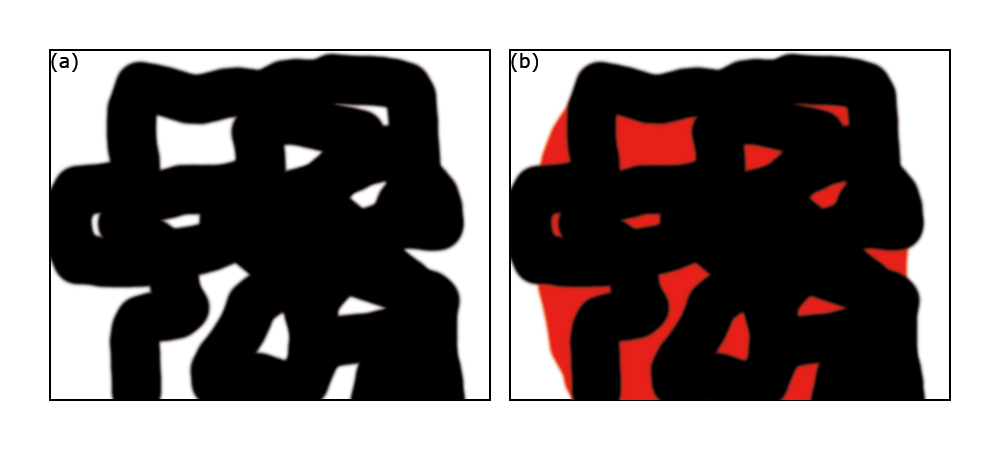
\includegraphics[width=0.9\textwidth, angle=0]{img/guided_exploration_1.png}
    \caption{(a) Karte nach der autonomen Erkundung (b) Der rote Bereich markiert das Gebiet, dass in der geführten Erkundung hinzukommen soll}
    \label{guidedexploration}
\end{figure}

Der Algorithmus verwendet die Daten vom Map-Modell und berechnet den Mittelpunkt aller bisher befahrenen Punkte. Von diesem Punkt ausgehend wird im Rotationsprinzip jeder Punkt der noch nicht befahren wurde ermittelt, wobei solange Punkte gesucht werden bis ein gewisser Schwellwert erreicht wird. Dieser Schwellwert kann abhängig von den Ausgangsbedingungen angepasst werden. Anschließend gibt es eine Menge von Punkten die Grundlage für die geführte Erkundung sind. Im nächsten Schritt wird die Menge aller Punkte in so viele Gebiete unterteilt wie es NXT's gibt. Ausgehend von der aktuellen Position der NXT's werden diese Gebiete zugeordnet und die NXT's fahren einzelne Punkte ab, um einen möglichst großen Teil der Ihnen zugeordneten Gebiete zu erkunden. Dabei kann nicht gefordert werden, dass die NXT's jeweils das ganze ihnen zugeordnete Gebiet erkunden, da nicht bekannt ist ob sich in den Bereichen Hindernisse befinden. Die Maßgabe für das erfolgreiche Beenden der Phase ist daher, dass das Ziel so wie ein Weg dorthin gefunden wurden. 

\subsection{Pfad zum Ziel}
%TODO Jonathan: Bilder-Pfade und Latex anpassen - das ist der Teil von Denis
\subsection*{Überblick}
	Im folgenden wird der Pathfinding Algorithmus näher beschrieben bei welchem aus einer erkundeten Karte und einem Start und Zielpunkt ein optimaler Pfad berechnet wird. Bedingungen hierfür sind jedoch eine erkundete Topologie. Übergeben wird diese als binärer Zweidimensionaler Array, sowie einem Startpunkt des Nao's und dem gefundenen Endpunkt. Der Algorithmus teilt sich in 3 Phasen: 
\begin{enumerate}
\item Die Breitensuche, die dafür sorgt ein gültigen Pfad vom Start, zum Endpunkt zu finden. 
\item Die Repositionierung des Pfades um ein möglichst großen Abstand zu den Hindernissen zu erreichen.
\item Die Pfadoptimierung, die eine Minimierung der Punkte zum Ziel hat. Das Resultat ist ein optimierter Pfad vom Start, zum Zielpunkt. Repräsentiert wird dieser durch eine Liste von Punkten.
\end{enumerate}

\subsection*{Breitensuche}
	Bei der Representation der Karte handelt es sich um ein 2-Deminsionallen Binären Array, wobei 1 für ein Hindernis stehen und 0 für einen Freifläche. Die Breitensuche geht nun folgendermaßen vor: Sie weist iterativ jedem Punkt die Entfernung zum Startpunkt zu. Dies geschieht indem jeder Punkt am Horizont, also der noch nicht betrachtet wurde und an einen bereits betrachteten Punkt grenzt, den Abstand des bisherigen Punktes + 1 annimmt. Dies geschieht so lange der Endpunkt noch nicht gefunden wurde. Ist ein Endpunkt gefunden Konstruiert man den Pfad vom Endpunkt zum Startpunkt aus, in dem jeweils immer der kleinste Folgepunkt dem Pfad hinzugefügt wird, bis man bei dem Startpunkt angekommen ist. Das Resultat ist ein Pfad an Punkten.\\
	\\

\begin{figure}[ht]
    \centering
	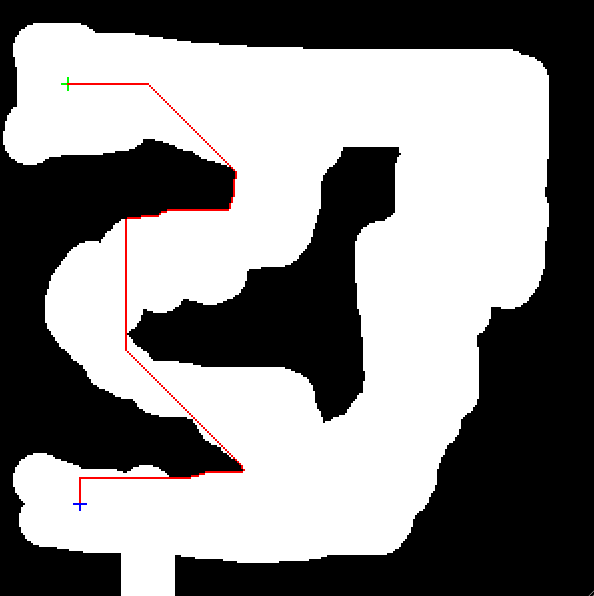
\includegraphics[width=0.35\textwidth, angle=0]{img/p2.png} 
\end{figure}
\subsection*{Repositioniertung}
	Die Breitensuche sollte nun einen Pfad zurückliefern. Dieser Pfad ist jedoch auf die minimale Distanz optimiert. Einen Roboter entlang dieses Pfades zu schicken ist nicht möglich, da der Pfad oft an möglichen Hindernissen langführt und die Breite der Roboter nicht berücksichtigt. Da die Position der Hindernisse auf der Karte auch einem Fehler unterliegen ist es sicherer den Roboter in der ``Mitte'' eines ``Ganges'' zu schicken. Die Repositionierung sträbt nun an aus dem Pfad der Breitensuche einen solchen optimalen Pfad an, der möglichst weit weg von möglichen hindernissen ist. Dazu wird durch jeden Punkt des Pfades 4 Linien geführt: Die Horizontale, Vertikale und beide Diagonalen, die jewels dort enden, wo diese an ein mögliches Hindernis stoßen. Um eine Abschätzung des Optimalen Punktes zu bekommen, wird nun der Mittelpunkt der kürzisten Linie genommen und aus ihr wird ein Kreis mit der Diagonale der Linie konstruiert. Das Ergebnis ist eine Menge M von Kreisen auf der Karte. \\


\begin{figure}[ht]
    \centering
	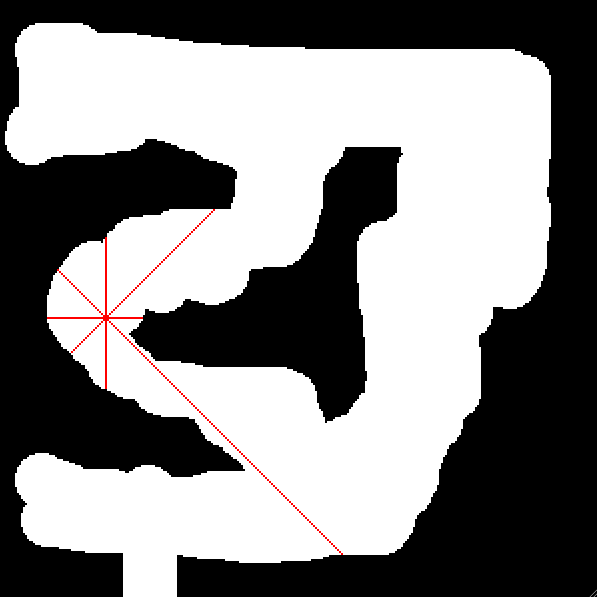
\includegraphics[width=0.35\textwidth, angle=0]{img/p3.png}
	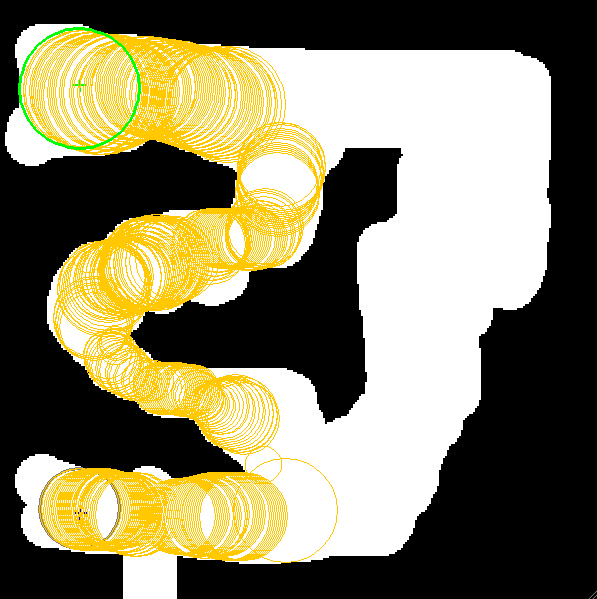
\includegraphics[width=0.35\textwidth, angle=0]{img/p4.png} 
\end{figure}

\subsection*{Optimierung}
	In der Optimierungsphase werden alle Kreise aus M, die sich überschneiden, miteinander verbunden. Das Ergebnis ist ein Graph. Auf dem resultierendem Graphen wird nun noch einmal eine Breitensuche vorgenommen, wobei die Länge der Verbindung mit einberechnet wird. Der resultierende Pfad aus dieser Breitensuche ist der gesuchte Pfad und wird zurückgegeben. \\
	
\begin{figure}[ht]
    \centering
	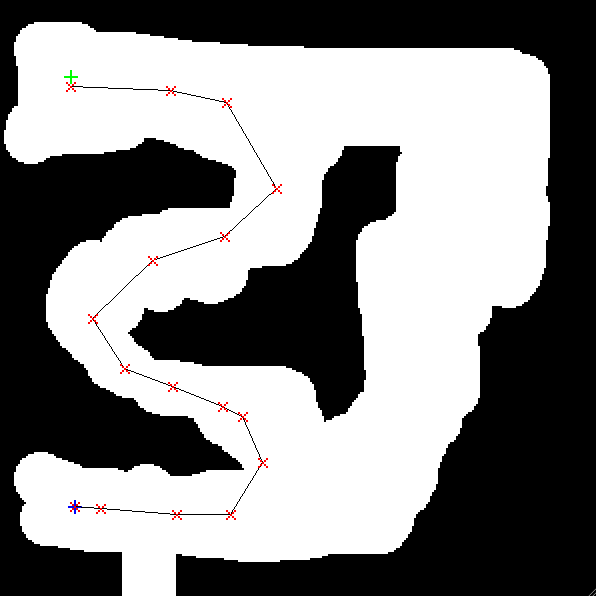
\includegraphics[width=0.35\textwidth, angle=0]{img/p5.png} 
\end{figure}